\documentclass[10pt,a4paper]{ieeeconf}
\usepackage[utf8]{inputenc}
\usepackage{amsmath}
\usepackage{amsfonts}
\usepackage{amssymb}
\usepackage{graphicx}
\usepackage{array}
\usepackage[thinlines]{easytable}
\usepackage{euler}
\usepackage{subcaption}
\usepackage{caption}
\usepackage[section]{placeins}
\usepackage{hyperref}
\usepackage[autostyle]{csquotes}
\usepackage{tikz}
\MakeOuterQuote{"}

\usepackage[backend=bibtex,sorting=none, urldate=edtf, date=edtf]{biblatex}
\addbibresource{bibfile.bib}

\usepackage{minted}

\begin{document}
  \title{
  COMP62https://www.kaggle.com/c/spooky-author-identification08 Advanced Machine Learning Group Report\\
  \vspace{5mm}
    Spooky Author Identification
  }
  \author{
    Tom Eccles \texttt{\href{mailto:tde1g14@soton.ac.uk}{tde1g14@soton.ac.uk}} \and
    George Elliott-Hunter \texttt{\href{mailto:gpeh1g14@soton.ac.uk}{gpeh1g14@soton.ac.uk}} \and \\
    Andrew Barrett-Sprot \texttt{\href{mailto:abs1g14@soton.ac.uk}{abs1g14@soton.ac.uk}} \and
    Lloyd Pearson \texttt{\href{mailto:lpp1g14@soton.ac.uk}{lpp1g14@soton.ac.uk}} \and
  }

  % make the title area
  \maketitle
  %\tableofcontents
  \begin{abstract}
    This report compares the effectiveness of various neural net and probabilistic techniques when applied to the Kaggle competition "Spooky Author Identification" \cite{kaggle}, in which three horror authors must be recognised by their writings. Overall a classification accuracy of 83\% and a loss of 0.43 is achieved using a combined neural net and bag-of-words approach.
  \end{abstract}
  
  \section{Introduction}
\label{sec:intro}
The Kaggle competition underling this work is "Spooky Author Identification", from December 2017. It challenges teams to classify sentences from the works of three
different horror authors. Classifiers were evaluatied by the log-loss metric.

Though the competition entry window had passed at the time of writing, the leaderboards may still be used to benchmark the performance of any classifiers.
  \section{Data Structure}
\label{sec:data_structure}
The data for this task is provided in two files: \textit{test.csv} and \textit{train.csv}. The training set contains approximately 20,000 labelled sentences, and the test set contains approximately 8,000 unlabelled sentences.

The data is provided in the form described in Table \ref{tab:data_form}.

\begin{table}[h]
\centering
\begin{tabular}{|c|c|c|}
\hline 
\textbf{id} & \textbf{text} & \textbf{author} \\ 
\hline 
id26305 & This process, however, afforded me \ldots & EAP \\ 
\hline 
id17569 & It never once occurred to me that \ldots & HPL \\ 
\hline 
\ldots & \ldots & \ldots \\ 
\hline 
\end{tabular} 
\caption{The provided data, as in \textit{test.csv}.}
\label{tab:data_form}
\end{table}
The three authors represented in this dataset are Edgar Allen Poe (\textit{EAP}), H.P Lovecraft (\textit{HPL}), and Mary Shelley (\textit{MWS}.

\subsection{Balanced Data}
\label{sec:balanced_data}

There is a slight bias in the dataset, but it is approximately balanced as shown in Figure \ref{fig:balance}. This should allow model training to work well without balancing of the training data.

\begin{figure}[h]
\centering
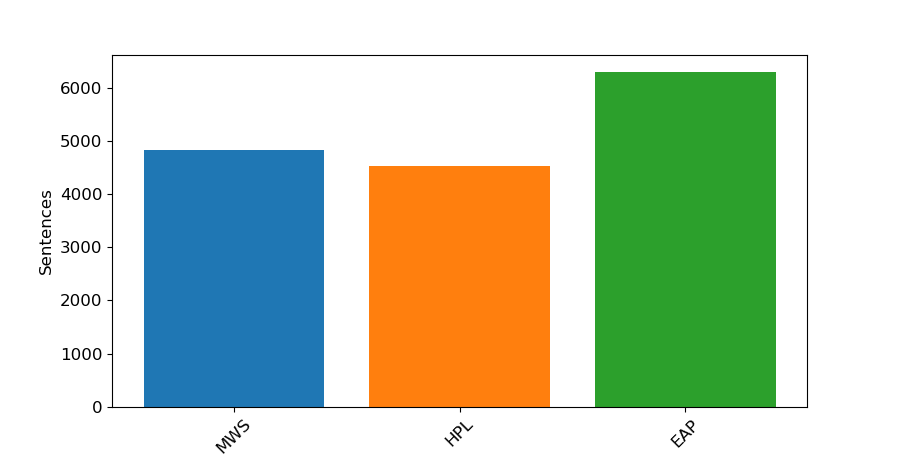
\includegraphics[width=0.6\textwidth]{Figures/Data_Structure/balance.png}
\caption{Number of sentences in the training set, by author}
\label{fig:balance}
\end{figure}

\subsection{Sentence Lengths}
\label{sec:sentence_lengths}

A broad examination of the data offers some insight into the difference between these authors' styles. The first and most obvious attribute to examine is the sentence length, which is shown in Figure \ref{fig:senlen}. Whilst the three authors are all largely similar in their distribution of sentence lengths, there is a noticeable difference. This may, therefore, provide a useful feature for discriminating between classes.

\begin{figure}[h]
\centering
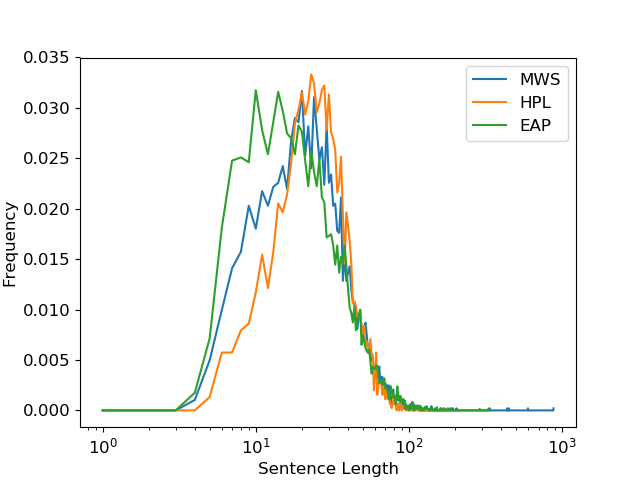
\includegraphics[width=0.9\textwidth]{Figures/Data_Structure/senlen.png}
\begin{tabular}{|c|c|c|}
\hline  
\textbf{Author} & \textbf{Mean} & \textbf{Standard Deviation} \\ 
\hline 
MWS & 31.3 & 26.0 \\ 
\hline 
HPL & 30.8 & 15.3 \\ 
\hline 
EAP & 29.4 & 21.1 \\ 
\hline 

\end{tabular} 
\caption{Sentence length frequency, by author}
\label{fig:senlen}
\end{figure}

\subsection{Word Frequency}
\label{sec:word_frequency}

Another obvious way in which the authors may differ is their word choice; They are likely to favour different words, and their occurrence in a sentence may evidence their author.

Figure \ref{fig:wordfreq_before} shows the most frequent words used by each author, and is not particularly useful; The majority of them are shared between authors. Removing stopwords produces the results in Figure \ref{fig:wordfreq_after}, which more uniquely identify the authors. At a glance these word sets don't seem to overlap a great deal, and so classifying sentences by the likelihood of each author to write it may be a productive approach.

\begin{figure}[h]
\centering
\begin{subfigure}[b]{0.49\textwidth}
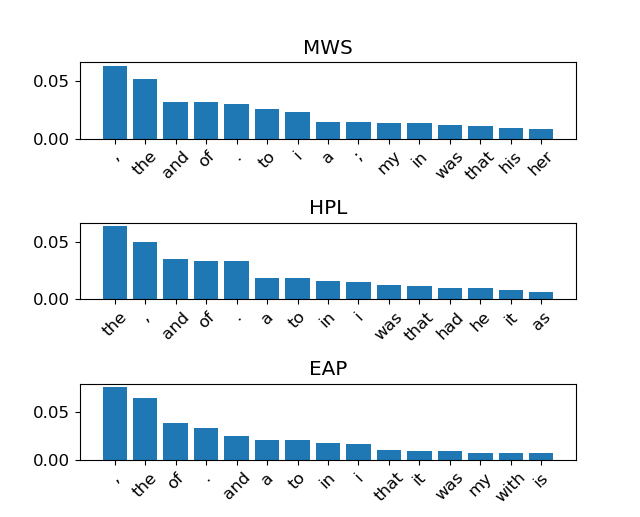
\includegraphics[width=\textwidth]{Figures/Data_Structure/wordfreq_before.png}
\caption{20 most used words, by author, before stopword removal}
\label{fig:wordfreq_before}
\end{subfigure}
\begin{subfigure}[b]{0.49\textwidth}
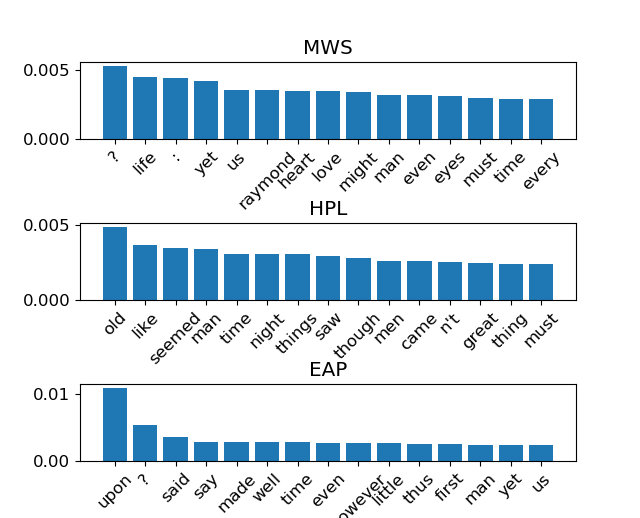
\includegraphics[width=\textwidth]{Figures/Data_Structure/wordfreq_after.png}
\caption{20 most used words, by author, after stopword removal}
\label{fig:wordfreq_after}
\end{subfigure}
\caption{Author word usage}
\label{fig:wordfreq}
\end{figure}


  \section{Data Processing}
\label{sec:data_processing}

  \subsection{Preprocessing}
  \label{sec:preprocessing}
    \textbf{Renamed from ``Pipelines''}

  \subsection{Word2Vec}
  \label{sec:word2vec}

  \subsection{Sentence Transformations}
  \label{sec:sentence_transformations}
    \textbf{Renamed from ``Padded vs Windowed''}

  \subsection{Label Encoding}
  \label{sec:label_encoding}
  
  \section{First Models}
\label{sec:first_models}

\subsection{Bag of Words}
\label{sec:bag_of_words}
From the examination of the data in Section \ref{sec:word_frequency}, a bag-of-words classifier seems plausible. Through a direct comparison of the frequencies with which each author uses the words in a given sentence, a prediction may be formed.

Let $\phi_w^a$ be the number of occurrences of some word $w$ in the corpus of sentences attributed to author $a$. The estimated probability of an author's usage of a word, $w^*$, is given by:

\begin{equation*}
p_{w*}^a = \frac{\phi_w^a}{\sum\limits_{w} \phi_w^a}
\end{equation*}

The estimated probability of a sentence, $s$, is given by:

\begin{align*}
p_{s}^a &= \prod\limits_{w\in s} p_{w}^a \\
log(p_{s}^a &)= \sum\limits_{w\in s} log(p_{w}^a)
\end{align*}

During prediction, however, it is likely that certain words will not have occurred in the training data: a "miss". An intuitive way to handle this is to score authors first on the number of words they "hit", and then by the probability of those words. Denoting the words used by each author in the training set as $W_a$ and the set of authors $A$, the following scoring mechanism is introduced:

\begin{align*}
score(s,a) &= \sum\limits_{w\in s}
\begin{cases}
log(p_{w}^a) & w\in W_a \\
0 & w \not\in W_a
\end{cases}\\
hits(s,a) &= \sum\limits_{w\in s}
\begin{cases}
1 & w\in W_a \\
0 & w \not\in W_a
\end{cases}\\
cands(s) &= a^* \in A : hits(s,a^*) = \max_a(hits(s,a))\\
winner(s) &= \underset{a}{\arg\max}(score(s,a))\quad \forall a \in cands(s)
\end{align*}

Running this model on the training set with 3 cross-validation passes (such that each third of the training data is predicted based on a model trained on the remaining two-thirds) yields the confusion matrix and accuracy in Table \ref{tab:bow_cw}. Log-loss metrics are not available for this model as it doesn't produce output probabilities, only binary classifications.

\begin{table}[h]
\centering
\begin{tabular}{m{1cm}|m{1cm}|m{1cm}|m{1cm}|m{0cm}}
\multicolumn{1}{m{1cm}}{} & \multicolumn{1}{m{1cm}}{EAP} & \multicolumn{1}{m{1cm}}{HPL} & \multicolumn{1}{m{1cm}}{MWS} &\\[5pt]
\cline{2-4}
EAP & 4910 & 630 & 760 & \\[5pt]
\cline{2-4}
HPL & 476 & 3774 & 283 & \\[5pt]
\cline{2-4}
MWS & 615 & 381 & 3834 & \\[5pt]
\cline{2-4}
\end{tabular}
\caption{Results for bag-of-words classifier, stemming and lemmatisation enabled.\\Accuracy: 80\%}
\label{tab:bow_cw}
\end{table}

\subsection{Forest}
\label{sec:forest}

\subsection{Windowed Neural Network}
In order to recognise tell-tale structures in the way sentences are composed, a classifier must be able to examine words in context. By running a window over the sentence tokens, this can be achieved.

Using a word embedding of $d$ dimensions, a window of $n$ words is provided as the input to a neural network. These words are flattened into a $d \times n$ wide layer, and fed through some number of hidden Relu units before being fed to a classifying output layer. This overall structure is described in Figure \ref{fig:win_nn_structure}.

\begin{figure}[h]
\def\layersep{2cm}
\begin{tikzpicture}[shorten >=1pt,->,draw=black!50, node distance=\layersep]
    \tikzstyle{every pin edge}=[<-,shorten <=1pt]
    \tikzstyle{neuron}=[circle,fill=black!25,minimum size=17pt,inner sep=0pt]
    \tikzstyle{input neuron}=[neuron, fill=green!50];
    \tikzstyle{output neuron}=[neuron, fill=red!50];
    \tikzstyle{hidden neuron}=[neuron, fill=blue!50];
    \tikzstyle{annot} = [text width=4em, text centered]

    % Draw the input layer nodes
    \foreach \name / \y in {1,...,4}
    % This is the same as writing \foreach \name / \y in {1/1,2/2,3/3,4/4}
        \node[input neuron, pin=left:Word \#\y] (I-\name) at (0,-\y) {};
        
    % Draw the hidden layer nodes
    \foreach \name / \y in {1,...,5}
        \path[yshift=0.5cm]
            node[hidden neuron] (H-\name) at (\layersep,-\y cm) {};

    % Draw the output layer node
    \foreach \name / \y in {1,...,3}
    	\path[yshift=-0.5cm]
            node[output neuron] (G-\name) at (2*\layersep,-\y cm) {};

    % Connect every node in the input layer with every node in the
    % hidden layer.
    \foreach \source in {1,...,4}
        \foreach \dest in {1,...,5}
            \path (I-\source) edge (H-\dest);

    % Connect every node in the hidden layer with the output layer
    \foreach \source in {1,...,5}
        \foreach \dest in {1,...,3}
            \path (H-\source) edge (G-\dest);

    % Annotate the layers
    \node[annot,above of=H-1, node distance=1cm] (hl) {Hidden Relu layer(s)};
    \node[annot,left of=hl] {Input Flatten layer};
    \node[annot,right of=hl] {Output Sigmoid layer};
\end{tikzpicture}
\caption{Windowed neural network structure}
\label{fig:win_nn_structure}
\end{figure}

The word embedding for this network may either be built on the training set itself or imported from a pre-trained model. The former may create a more subject-specific embedding since it is trained on relevant data; however the relatively small corpus size means that the spacial relationship between words may be weaker and the likelihood of missing words in the test data may be higher.

For this classifier, these embeddings are as described in Section \ref{sec:word2vec}.

In either case, it must be decided how to deal with words in the test data that do not exist in the word embedding. For the embedding built from the training set, unique words (that is, words that appear only once across all sentences) are replaced with a \textit{RARE} token. This creates an embedding for unique words, and when the model is run any words which do not exist in the embedding may be replaced with this token.

For the pre-trained model, inserting tokens is not possible. Instead words that do not exist within the embedding are replaced with a mean vector, $\vec{e}_{rare}$, derived from the embedding $E$, such that:

\begin{equation*}
\vec{e}_{rare} = \frac{1}{\lVert E \rVert} \sum\limits_{\vec{w} \in E}^{\lVert E \rVert} \vec{w}
\end{equation*}


Additionally test sentences with length less than the window size must be padded to at least that length; In this model, such sentences are being appended with the last word in the sentence until long enough.

The confusion matrices, log-losses and accuracies for this model under both encoder methods are shown in Table \ref{tab:window_res}.

\begin{table}[h]
\centering
\begin{subtable}{\columnwidth}
\centering
\begin{tabular}{m{1cm}|m{1cm}|m{1cm}|m{1cm}|m{0cm}}
\multicolumn{1}{m{1cm}}{} & \multicolumn{1}{m{1cm}}{EAP} & \multicolumn{1}{m{1cm}}{HPL} & \multicolumn{1}{m{1cm}}{MWS} &\\[5pt]
\cline{2-4}
EAP & 4504 & 773 & 1023 & \\[5pt]
\cline{2-4}
HPL & 1201 & 2632 & 700 & \\[5pt]
\cline{2-4}
MWS & 1206 & 543 & 3081 & \\[5pt]
\cline{2-4}
\end{tabular}
\caption{Encoding built from training data, stemming and lemmatisation enabled.\\Loss: 1.83 Accuracy: 65%}
\end{subtable}\\
\vspace{1cm}
\begin{subtable}{\columnwidth}
\centering
\begin{tabular}{m{1cm}|m{1cm}|m{1cm}|m{1cm}|m{0cm}}
\multicolumn{1}{m{1cm}}{} & \multicolumn{1}{m{1cm}}{EAP} & \multicolumn{1}{m{1cm}}{HPL} & \multicolumn{1}{m{1cm}}{MWS} &\\[5pt]
\cline{2-4}
EAP & 4587 & 757 & 956 & \\[5pt]
\cline{2-4}
HPL & 1084 & 2885 & 564 & \\[5pt]
\cline{2-4}
MWS & 1019 & 525 & 3286 & \\[5pt]
\cline{2-4}
\end{tabular}
\caption{Pre-trained GloVe encoder, stemming and lemmatisation enabled.\\Loss: 1.90 Accuracy: 69%}
\end{subtable}
\caption{Results for windowed neural net classifier.}
\label{tab:window_res}
\end{table}

\label{sec:dnn}

\subsection{RNN}
\label{sec:rnn}
  \section{Extensions}
\label{sec:extensions}
  
\subsection{Beta Distribution Bag-of-words}
\label{sec:bow_beta}
The bag-of-words model described in Section \ref{sec:bag_of_words} has some substantial issues regarding the probability estimates $p_w^a$. Most notably is its bias towards words which occur only very few times, and only with a single author.

A good example is the word "marker". In the training set Lovecraft uses it exactly once, but both Shelly and Poe don't use it at all. Is it fair for this to be considered a "signature word" for Lovecraft? It could simply be that each author uses it with a similar frequency and it just happens that it was only observed once.

A better estimate for the usage probabilities can be provided by beta distributions, which provide a probability distribution for the actual occurrence rate of an event. By making some assumptions and simplifications - such as the usage of words by an author being independent of one another and a uniform prior distribution - it is possible to easily form this revised estimate. While these simplifications are obviously not a complete reflection of the real world, the posterior probability given by this model is likely to still be an improvement over that in Section \ref{sec:bag_of_words}.

The beta distribution is denoted by $Beta(\alpha , \beta)$ and has its mean at $\mathbb{E}(Beta(\alpha, \beta)) = \frac{\alpha}{\alpha + \beta}$. For $n$ random, independent trials with a uniform prior in which some outcome $x$ occurs $s$ times, the posterior probability is given by:

\begin{equation*}
p(x) = Beta(\alpha + s, \beta + n - s)
\end{equation*}

And has expectation:
\begin{equation*}
\mathbb{E}(p(x)) = \frac{\alpha+s}{\alpha + \beta + n}
\end{equation*}

This can be used to form a new estimation for the word frequency for each author that doesn't unduly favour extremely rare words. Additionally, this formula still holds even when a word has not been observed in an author's vocabulary. Because of this the hierarchical scoring system presented in Section \ref{sec:bag_of_words} is not necessary and a direct comparison of probabilities between each author may be made. This also allows loss to be calculated.

Utilising this new metric the confusion matrix , accuracy and loss are as in Table \ref{tab:beta_res}.

\begin{table}[h]
\centering
\begin{tabular}{m{1cm}|m{1cm}|m{1cm}|m{1cm}|m{0cm}}
\multicolumn{1}{m{1cm}}{} & \multicolumn{1}{m{1cm}}{EAP} & \multicolumn{1}{m{1cm}}{HPL} & \multicolumn{1}{m{1cm}}{MWS} &\\[5pt]
\cline{2-4}
EAP & 4657 & 675 & 968 & \\[5pt]
\cline{2-4}
HPL & 286 & 3914 & 333 & \\[5pt]
\cline{2-4}
MWS & 285 & 316 & 4229 & \\[5pt]
\cline{2-4}
\end{tabular}
\caption{Results for bag-of-words classifier with beta distributions, stemming and lemmatisation enabled.\\Loss 3.34 Accuracy: 82\% }
\label{tab:beta_res}
\end{table}


  \subsection{Bag-of-words Feature Kernel Neural Net}
  \label{sec:bow_nn}
  The bag-of-words predictors described in Sections \ref{sec:bag_of_words} and \ref{sec:bow_beta} perform excellently in terms of accuracy, but the loss (observable only when utilising beta distributions) is very poor. Conversely the windowed neural net predictor in Section \ref{sec:win_nn} has a comparably poor accuracy but performs vastly better with regards to loss.
  
  This is because the neural network is directly trained against the loss function, whereas the bag-of-words models are not. Combining these two approaches -- the simplicity of a bag-of-words model with the loss-optimising nature of a neural net -- is likely to provide the best of both worlds with regards to loss and accuracy metrics.
  
  The beta-distribution bag-of-words predictor utilises solely the product of probabilities to form its prediction. While a classifier could be built on top of this alone, more metrics may be offered as input to improve performance. In this case the following are provided to the input layer, for each author:
  
  \begin{itemize}
  \item The mean log probability of all words \footnote{For any given sentence, this is simply a length-scaled version of the log likelihood. However by taking the mean, the magnitude of these variables is not dependent on sentence length}
  \item The max and min log probability of all words
  \item The standard deviation of log probabilities of all words
  \item The number of "missed" words in the sentence \footnote{"Missed" words are those not observed as having been used by an author in the training set. Whilst they are still assigned a probability as in Section \ref{sec:bow_beta}, their record as having been missed is retained}
  \end{itemize}
  
 Additionally, the sentence length is included based on the observations in Section \ref{sec:sentence_lengths}. This provides a 16 neuron input-layer.
 
 The confusion matrix, accuracy and loss for this model may be seen in Table \ref{tab:bow_nn_res}. The results presented utilise a perceptron with no hidden layers; adding hidden layers does not improve performance. Noticeable overfitting is observed with this architecture. Its training loss is $<0.2$, and its training accuracy $>90\%$. Attempts to overcome this such as compressing the model through a 2-neuron layer and increasing batch sizes were not successful.
  
\begin{table}[h]
\centering
\begin{tabular}{m{1cm}|m{1cm}|m{1cm}|m{1cm}|m{0cm}}
\multicolumn{1}{m{1cm}}{} & \multicolumn{1}{m{1cm}}{EAP} & \multicolumn{1}{m{1cm}}{HPL} & \multicolumn{1}{m{1cm}}{MWS} &\\[5pt]
\cline{2-4}
EAP & 3747 & 550 & 236 & \\[5pt]
\cline{2-4}
HPL & 419 & 5300 & 581 & \\[5pt]
\cline{2-4}
MWS & 286 & 582 & 3962 & \\[5pt]
\cline{2-4}
\end{tabular}
\caption{Results for bag-of-words feature kernel neural net, stemming and lemmatisation enabled.\\Loss 0.46 Accuracy: 83\% }
\label{tab:bow_nn_res}
\end{table}
  
  \subsection{Grid Searching}
  \label{sec:grid_search}

  \subsubsection{RNN}
  \label{sec:rnn_grid_search}

  \subsection{Ensemble}
  \label{sec:ensemble}
  
  \subsection{Translation}
  \label{sec:translation}
  To try and improve the results from some of the classifiers the data an enhanced data set was created. To create the enhanced data set the original sentences were translated to and from an alternative language. This is from suggestions from a differing Kaggle competition 'Toxic Comments' \cite{Jigsaw2017}. 
  
  The thought of doing this is as the sentences are very short we can get a more data to perform analysis on. To do this \textit{TextBlob} was used to translate the sentences in to German, Spanish and French and then back from each respective language into English. 
  
  Although an issue may be that some style lost in translation, it appears as though there is some enhancement in the loss by using translations of around 0.03 with the Bag-of-words Feature Kernal Neural Net as seen in the Table \ref{tab:bow_nn_res_tran}. The translation may also help prevent the over fitting that is seen without it.
  
 begin{table}[h]
\centering
\begin{tabular}{m{1cm}|m{1cm}|m{1cm}|m{1cm}|m{0cm}}
\multicolumn{1}{m{1cm}}{} & \multicolumn{1}{m{1cm}}{EAP} & \multicolumn{1}{m{1cm}}{HPL} & \multicolumn{1}{m{1cm}}{MWS} &\\[5pt]
\cline{2-4}
EAP & 0.82561218 & 0.12039488 & 0.05399294 & \\[5pt]
\cline{2-4}
HPL & 0.06722222 & 0.84674603 & 0.08603175 & \\[5pt]
\cline{2-4}
MWS & 0.05424431 & 0.1199793 & 0.8257764 & \\[5pt]
\cline{2-4}
\end{tabular}
\caption{Results for bag-of-words feature kernel neural net, stemming and lemmatisation enabled, using a translated enhanced data set.\\Loss 0.43 Accuracy: 83\% }
\label{tab:bow_nn_res_tran}
\end{table}

  \subsection{kPCA}
  \label{sec:kpca}
    An attempt was made to use kernel principal component analysis (kPCA) to help to produce more separable data. To do this a kPCA was used on a Count Vectorizer and a Term Frequency – Inverse Document Frequency Vectorizer.
    
  \begin{figure}[h]
    \centering
    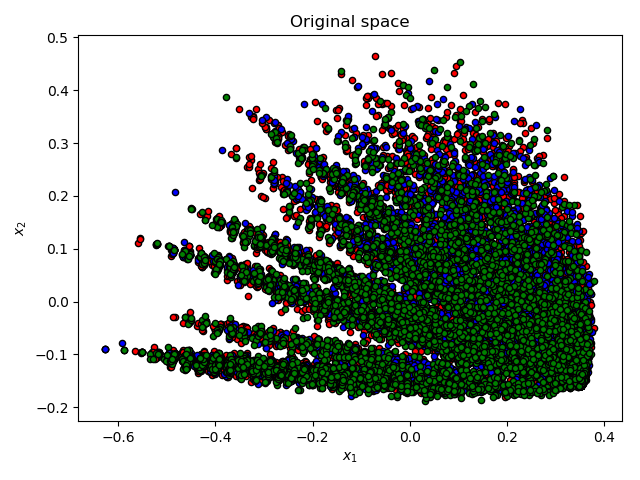
\includegraphics[width=\columnwidth]{Figures/Extensions/kPCALemmaRBF.png}
    \caption{kPCA performed on a Lemma Count Vectorizer using RBF kernel and a gamma of 0.04}
    \label{fig:balance}
  \end{figure}
  

  \section{Conclusion}
\label{sec:conclusion}
  \section{Future Work}
\label{sec:future_work}
    
  \printbibliography
  
  %\appendix
\end{document}
